\section{Implementation}

The approach to this project can be broken into a couple of different main parts. First, we need to find the location of both the object to pick up and the location where the object should be placed. Once the locations are found they need to be transformed from the camera coordinate frame to the base frame of the robot arm. Finally, we have all the information that the robot arm needs to move to the object, pick it up, move to the drop-off location, and put the object down.

\subsection{Localization and Transformation}

For our project, the main focus and innovation was the fact that we used AprilTags to allow dynamic object and drop-off locations. We were unable to get the AprilTags working within the Simulink code but could run it in a separate Matlab script. This was because the code to identify and localize the AprilTags was too slow and seemed to be a blocking call which interrupted the communication of Simulink with the arm when used inside the Simulink Model. To get around this we used the Simulink model to save a picture to disk, as shown in Figure \ref{Fig:QARM_CamPic}, then manually ran the Matlab script to determine the locations of the Object and Drop-off point. The Matlab Script then called the readAprilTag() function to retrieve the pose of each of the tags in its field of view along with an ID of the tag that matches the specific pattern of the tag. These IDs are then matched to the known values we are looking for to the Object's tag ID and the Drop-off point's tag ID. The final step for localization is that the user manually copies the locations from the Matlab Output and puts them in their respective input boxes in Simulink. The locations are with respect to the camera's frame.

\begin{figure}[htb]
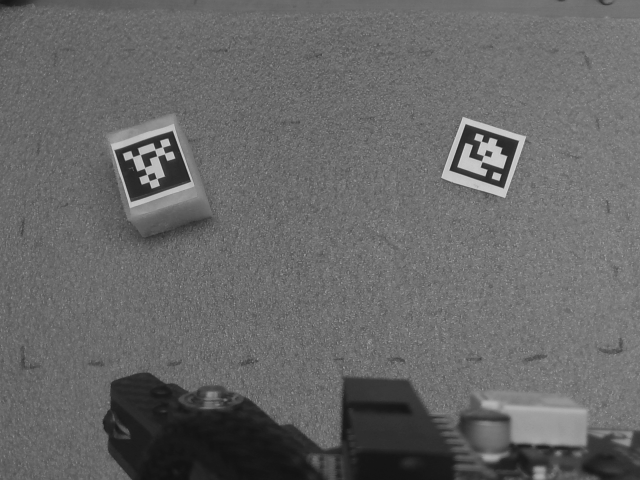
\includegraphics[width=8cm]{Figures/Input.png}
\caption{QArm Camera Input Picture with Object (left) and Drop-off (right)}
\centering
\label{Fig:QARM_CamPic}
\end{figure}

In order to transform the locations of the object and dropoff point from the camera's coordinate frame to the base frame we first transformed the locations to the wrist frame and then used forward kinematics to determine the transform from the wrist to the base. This allowed us to use the locations of the object and dropoff point relative to the base to then use inverse kinematics to determine what commands to send the robot to reach the locations commanded.

\subsection{Motion Planning}

Once the locations of the object and the drop-off point are inserted the model can then use them to pick up the object, move to the drop-off location, and put the object down. This was achieved by using a counter which started when the model was put into the Execute state(Value 3 at the top) that controls which location the arm is supposed to be at. It also sets the state of the gripper by switching the input to the corresponding state. The gripper itself is on a 1-second delay to allow the arm to reach the commanded position before it changes to allow the arm to reach the object and the dropoff point before closing or opening. This is done in a sequence of going to the location above the object, moving to the object and closing the gripper, moving back up, moving above the goal, moving to the goal and opening the gripper, and finally moving back up. These locations were calculated by taking the object position and the dropoff position in the base frame and for the locations above each location adding an offset.

